\documentclass[a4paper,12pt]{article}
\usepackage{amsmath,amsfonts,amsthm,amssymb, mathtools,steinmetz, gensymb, siunitx}	% LOADS USEFUL MATH STUFF
\usepackage{xcolor,graphicx}
\usepackage[left=1cm, top=2cm, right=1cm, bottom=1cm ,a4paper]{geometry} 				% ADJUSTS PAGE
\usepackage{setspace}
\usepackage{caption}
\usepackage{tikz}
\usepackage{pgf,tikz,pgfplots}
\usepackage{mathrsfs}
\usepackage{fancyhdr}
\usepackage{float}
\usepackage{array}
\usepackage{unicode-math}
\usepackage{booktabs}
\setmathfont{Libertinus Math}

\usetikzlibrary{decorations.pathreplacing,decorations.markings}
\usepgfplotslibrary{fillbetween}

\newcommand{\defeq}{\vcentcolon=}
\newcommand\block[1]{\hspace*{#1}}
\newcommand{\rpm}{\sbox0{$1$}\sbox2{$\scriptstyle\pm$}
	  \raise\dimexpr(\ht0-\ht2)/2\relax\box2 }
\pgfplotsset{compat=1.11}
	  
\newlength{\QNo}
\settowidth{\QNo}{2.}

\newlength{\QLetter}
\settowidth{\QLetter}{(a)}

\pagestyle{fancy}
\rhead{CS Honours Machine Learning}
\lhead{J L Gouws}

\begin{document}
\fontencoding{T1}
\fontfamily{ppl}\selectfont
\thispagestyle{empty}

{\Large \textbf{Assignment 1 ML}} \hfill {\Large \textbf{J L Gouws}}\\
\block{1.0cm} {\large \textbf{\today}} \hfill {\large \textbf{19G4436}}\\

1. See script file for details.
\begin{figure}[H]
  \centering
  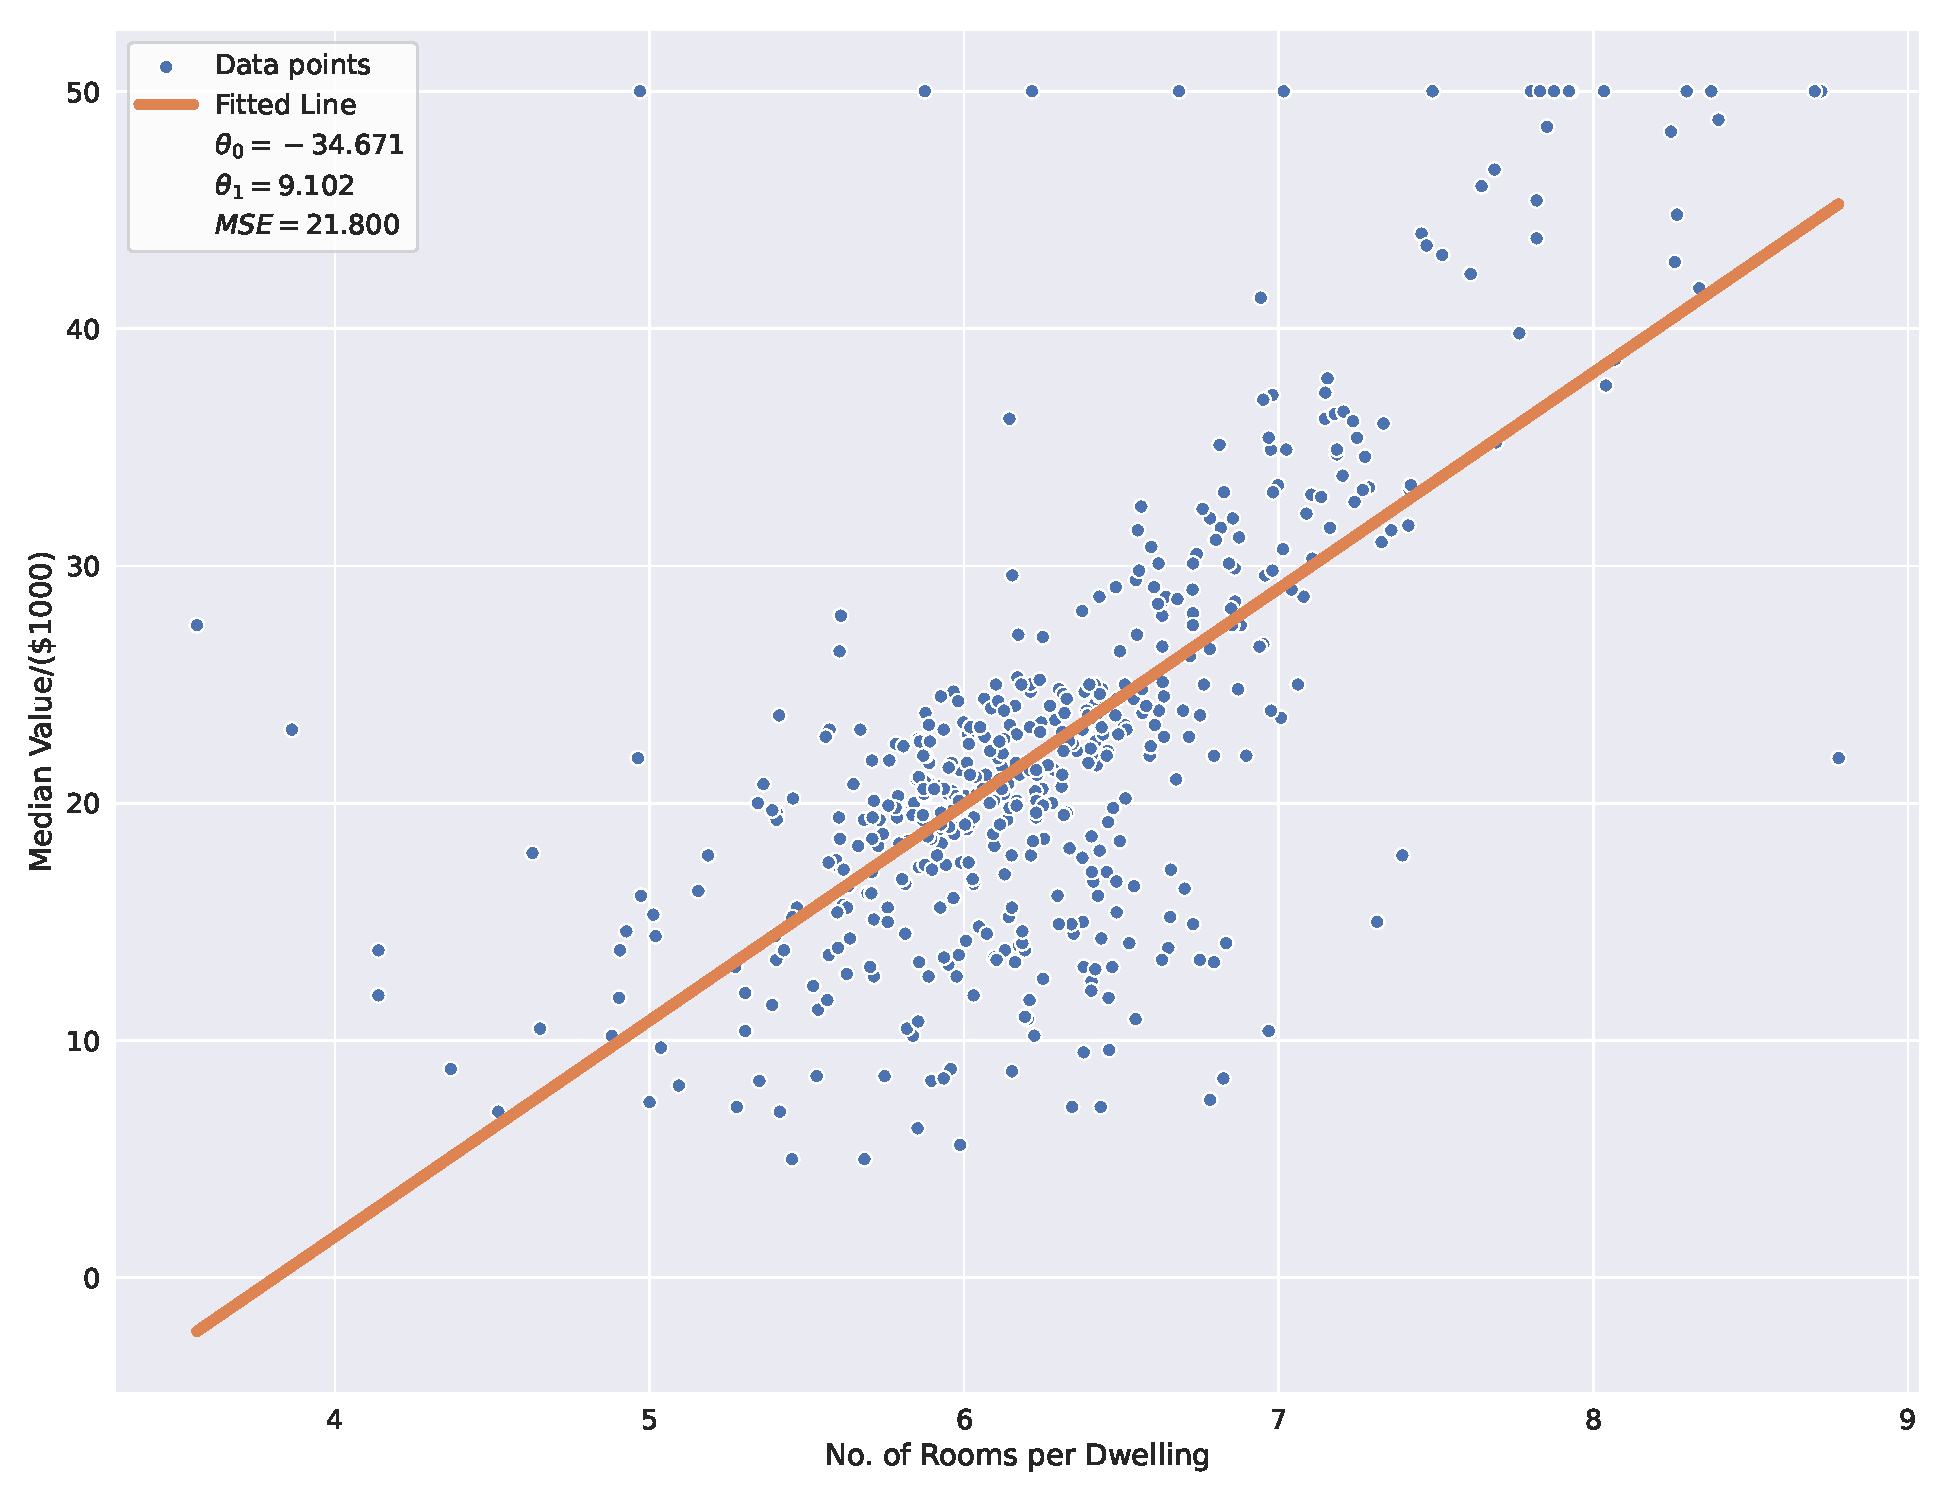
\includegraphics[scale = 0.4]{Task1/RMvsMEV.pdf}
  \caption{The relation between RM and MEDV with a fitted regression line.}
\end{figure}

2. 
\begin{minipage}[t]{0.90\dimexpr\textwidth}
  a)
  \begin{minipage}[t]{\dimexpr\textwidth}
    See script file.\\
  \end{minipage}

  b)
  \begin{minipage}[t]{\dimexpr\textwidth-\QNo}
    It is pretty much the same, the testing errors are the same to the first four significant figures.\\
    This can be seen by looking at the $MSE$(on test data) in Table~\ref{tab:models}.\\
  \end{minipage}

  c)
  \begin{minipage}[t]{\dimexpr\textwidth-\QNo}
    The plot of the two graphs is also more or less the same.\\
    The plot for Lasso regression is significantly different, however.\\
    We can see the values of the parametes of the two variables in Table~\ref{tab:modelsParams}.
    We can see the difference in the training methods for the Bivariate case in Figure~\ref{fig:bivModels}.\\
  \end{minipage}

  d)
  \begin{minipage}[t]{\dimexpr\textwidth-\QNo}
    The normal linear model seemed to train faster, but the Ridge model's test went faster.
    That being said, the difference in testing speed could be down to random error.
    There are other processes running on my computer which might interfere with accurate timing\\
  \end{minipage}

  e)
  \begin{minipage}[t]{\dimexpr\textwidth-\QNo}
    Yes, the Lasso method has a significantly larger MSE, and the model also trained a lot slower.\\
  \end{minipage}

  f)
  \begin{minipage}[t]{\dimexpr\textwidth-\QNo}
    We can see in Table~\ref{tab:models}, Table~\ref{tab:modelsA2} and Table~\ref{tab:modelsA3} that the $MSE$ does change as Lasso and Ridge parameter changes.
    The generalization error actually increases as we change the parameters.
    The training and testing times do not change, however.\\
  \end{minipage}

  g)
  \begin{minipage}[t]{\dimexpr\textwidth-\QNo}
    The mean absolute error:\\
    \begin{equation*}
      MAE = \frac{1}{n}\sum_{i=1}^n|y_i -\hat y_i|
    \end{equation*}
    This is very similar to the MSE. Only the errors are not squared.
    For MSE, squaring a large absolute error makes the error disproportionately large, which punishes an outliers.
    Since large errors are not squared for MAE, the outliers are punished but not over excessively.\\
  \end{minipage}

  h)
  \begin{minipage}[t]{\dimexpr\textwidth-\QNo}
    The adjusted $R^2$ metric tries to deal with this problem, the formula is:
    \begin{equation*}
      R^2_{\text{adj}} = 1 - \frac{(1 - R^2)(N - 1)}{N - p - 1}
    \end{equation*}
    Where $N$ is the total sample size, and $p$ is the number of features of the model.\\
  \end{minipage}

  i)
  \begin{minipage}[t]{\dimexpr\textwidth-\QNo}
    We cannot compare this to the results of Task 1.
    Task 1 is a bivariate linear regression and does not depend on B.\\

    We can compare this to part a) for the multi-linear case.
    We can see the difference in the parameters when `B' is dropped by comparing Table~\ref{tab:modelsParams} and Table~\ref{tab:modelsParamsExcB}.
    We can see that the multidimensional plot changes for the multilinear case, MEDV depends differently on RM.
  \end{minipage}
\end{minipage}
\begin{table}[H]
\centering
\caption{Different Linear Regression Models}
\label{tab:models}
\begin{tabular}{ccccc}
\toprule
Model & MSE & $R^2$ & Train Time $\times 10^{-6}$ & Test Time $\times 10^{-6}$ \\
\midrule
Linear & 22.737590 & 0.759814 & 368.595123 & 74.386597 \\
Ridge & 22.923754 & 0.763344 & 409.841537 & 68.187714 \\
Lasso & 27.606505 & 0.701360 & 460.863113 & 71.048737 \\
\bottomrule
\end{tabular}
\end{table}

\begin{table}[H]
\centering
\caption{Parameters of Different Linear Regression Models}
\label{tab:modelsParams}
\begin{tabular}{ccccccccccccccc}
\toprule
Model & $\theta_0$ & $\theta_{1}$ & $\theta_{2}$ & $\theta_{3}$ & $\theta_{4}$ & $\theta_{5}$ & $\theta_{6}$ & $\theta_{7}$ & $\theta_{8}$ & $\theta_{9}$ & $\theta_{10}$ & $\theta_{11}$ & $\theta_{12}$ & $\theta_{13}$ \\
\midrule
Linear & 36.73 & -0.12 & 0.04 & 0.02 & 2.78 & -18.59 & 3.76 & 0.00 & -1.47 & 0.31 & -0.01 & -0.95 & 0.01 & -0.55 \\
Ridge & 31.47 & -0.12 & 0.04 & -0.01 & 2.57 & -10.79 & 3.80 & -0.00 & -1.36 & 0.30 & -0.01 & -0.86 & 0.01 & -0.56 \\
Lasso & 40.55 & -0.08 & 0.04 & -0.00 & 0.00 & -0.00 & 1.01 & 0.02 & -0.64 & 0.27 & -0.01 & -0.74 & 0.01 & -0.78 \\
\bottomrule
\end{tabular}
\end{table}

\begin{table}[H]
\centering
\caption{Different Linear Regression Models when B is Excluded}
\label{tab:models}
\begin{tabular}{ccccc}
\toprule
Model & MSE & $R^2$ & Train Time $\times 10^{-6}$ & Test Time $\times 10^{-6}$ \\
\midrule
Linear & 23.425683 & 0.775628 & 464.200974 & 53.882599 \\
Ridge & 23.628806 & 0.777696 & 337.362289 & 51.975250 \\
Lasso & 28.433794 & 0.710581 & 428.676605 & 56.266785 \\
\bottomrule
\end{tabular}
\end{table}

\begin{table}[H]
\centering
\caption{Parameters of Different Linear Regression Models With B Excluded}
\label{tab:modelsParamsExcB}
\begin{tabular}{ccccccccccccccc}
\toprule
Model & $\theta_0$ & $\theta_{1}$ & $\theta_{2}$ & $\theta_{3}$ & $\theta_{4}$ & $\theta_{5}$ & $\theta_{6}$ & $\theta_{7}$ & $\theta_{8}$ & $\theta_{9}$ & $\theta_{10}$ & $\theta_{11}$ & $\theta_{13}$ \\
\midrule
Linear & 42.31 & -0.13 & 0.04 & 0.01 & 2.98 & -19.42 & 3.59 & 0.01 & -1.48 & 0.29 & -0.01 & -0.93 & -0.58 \\
Ridge & 36.95 & -0.13 & 0.04 & -0.02 & 2.77 & -11.28 & 3.64 & 0.00 & -1.37 & 0.27 & -0.01 & -0.84 & -0.59 \\
Lasso & 45.02 & -0.09 & 0.04 & -0.00 & 0.00 & -0.00 & 0.88 & 0.03 & -0.64 & 0.26 & -0.02 & -0.72 & -0.81 \\
\bottomrule
\end{tabular}
\end{table}

\begin{table}[H]
\centering
\caption{Different Linear Regression Models with $\alpha = 2$}
\label{tab:modelsA2}
\begin{tabular}{ccccc}
\toprule
Model & MSE & $R^2$ & Train Time $\times 10^{-6}$ & Test Time $\times 10^{-6}$ \\
\midrule
Linear & 22.737590 & 0.759814 & 406.980515 & 68.664551 \\
Ridge & 23.108689 & 0.762833 & 329.732895 & 66.995621 \\
Lasso & 32.515507 & 0.639673 & 385.046005 & 69.856644 \\
\bottomrule
\end{tabular}
\end{table}

\begin{table}[H]
\centering
\caption{Different Linear Regression Models with $\alpha = 3$}
\label{tab:modelsA3}
\begin{tabular}{ccccc}
\toprule
Model & MSE & $R^2$ & Train Time $\times 10^{-6}$ & Test Time $\times 10^{-6}$ \\
\midrule
Linear & 22.737590 & 0.759814 & 388.145447 & 67.710876 \\
Ridge & 23.237427 & 0.761974 & 329.017639 & 66.518784 \\
Lasso & 34.971519 & 0.623029 & 356.912613 & 70.095062 \\
\bottomrule
\end{tabular}
\end{table}


\begin{figure}[H]
  \centering
  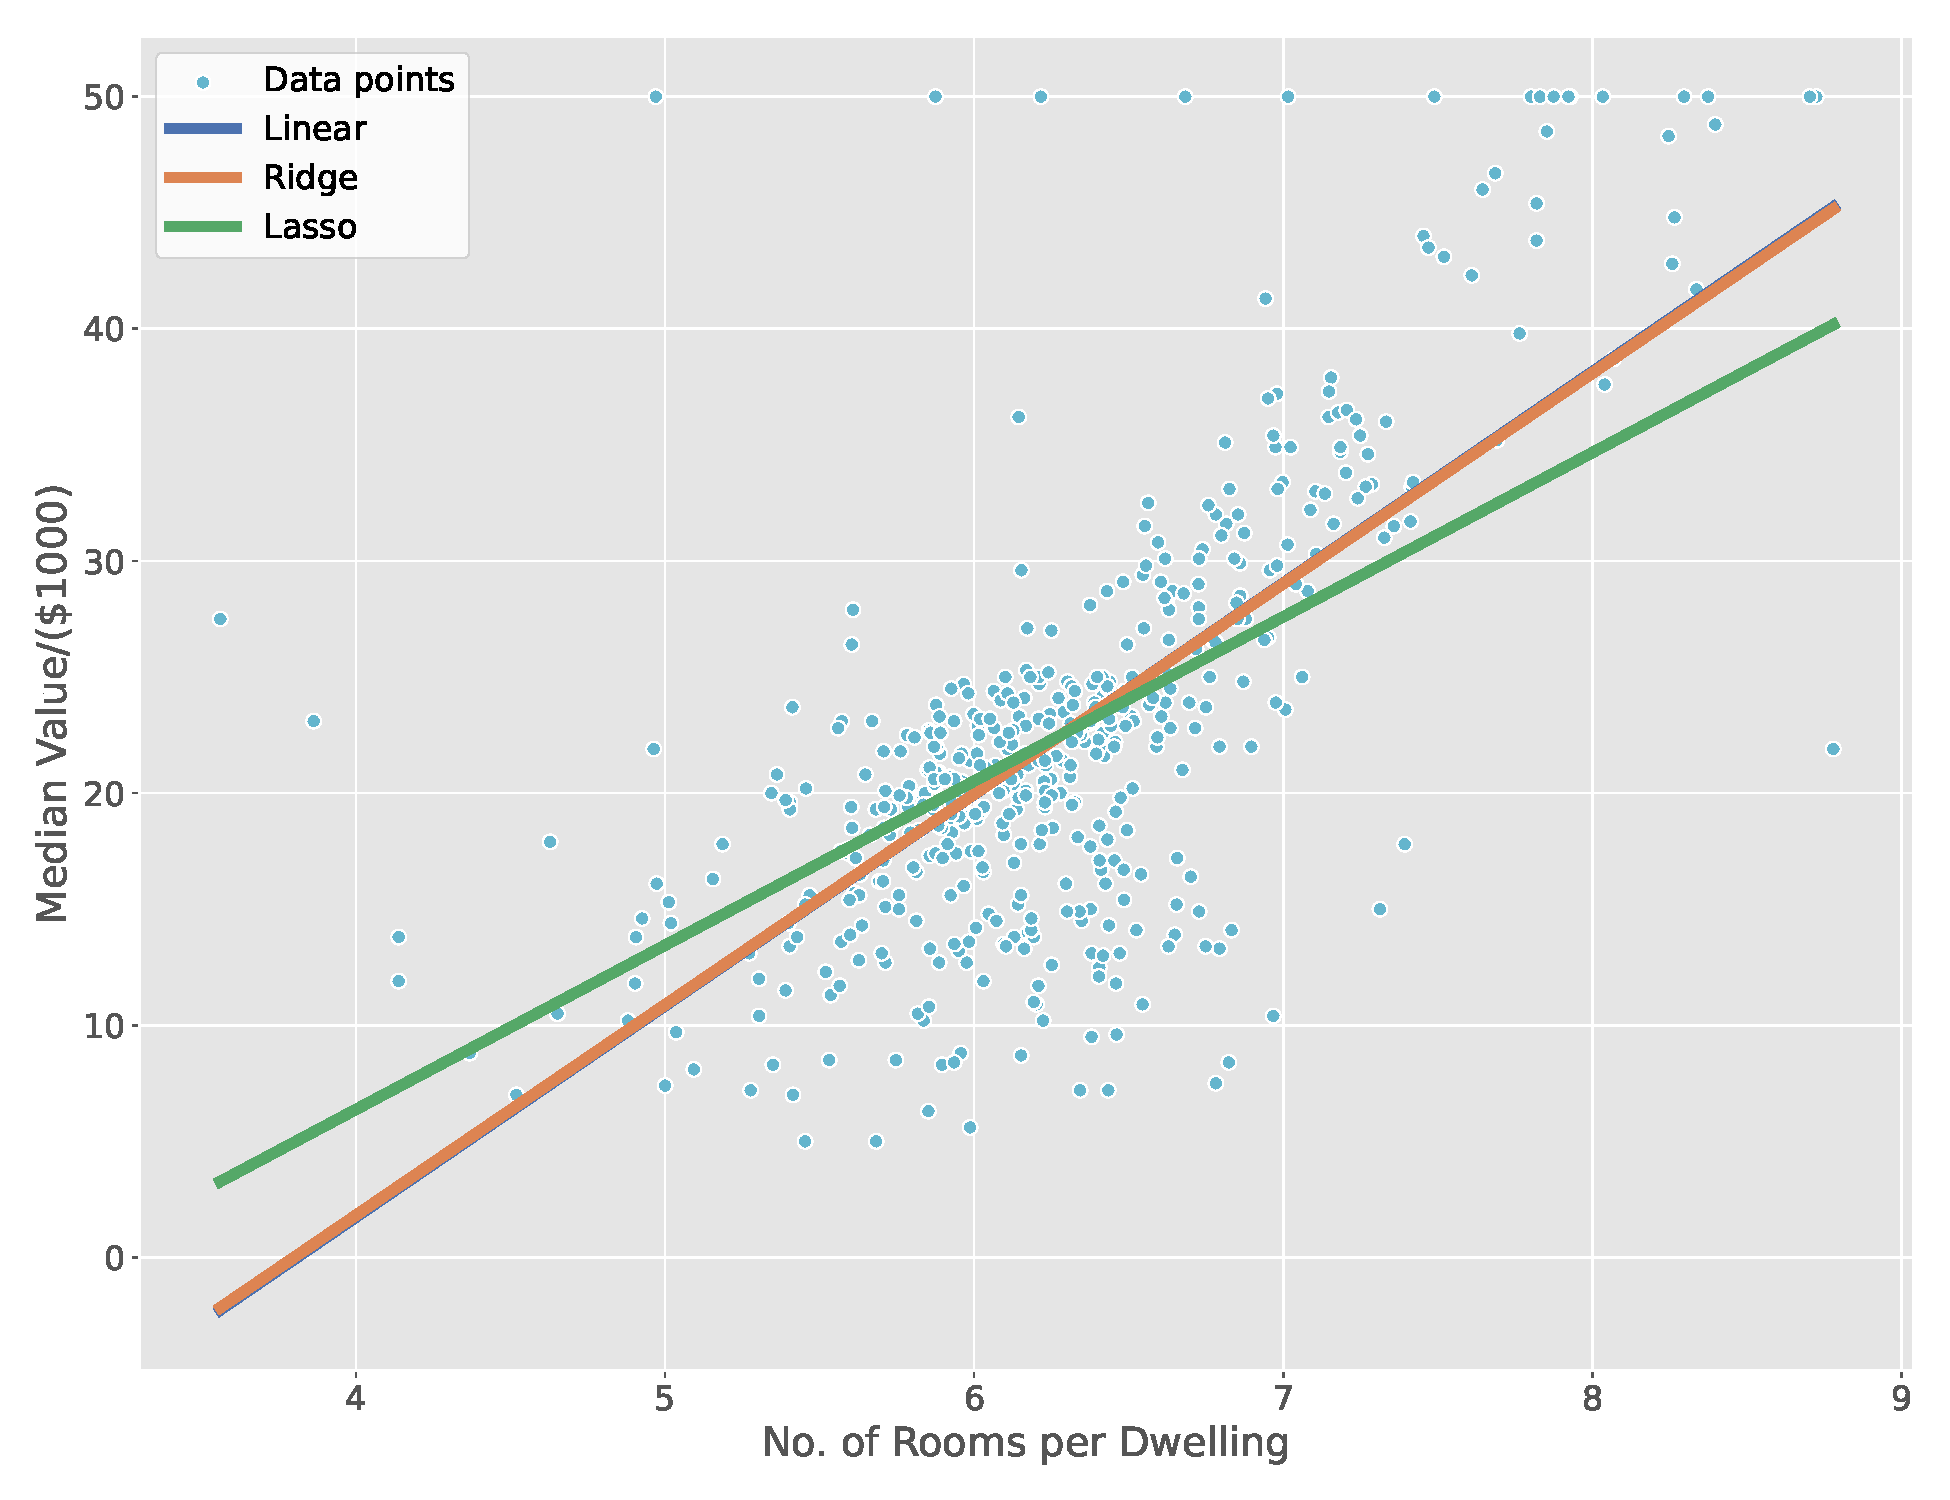
\includegraphics[scale = 0.4]{Task2/RMvsMEVBivariate.pdf}
  \caption{The relation between RM and MEDV for different regression methods.}
  \label{fig:bivModels}
\end{figure}

3 and 4. 
\begin{minipage}[t]{0.8\dimexpr\textwidth}
  A quick note on the results.
  The classifier for task 3 and task 4 has an accuracy of $100\%$.
  This makes sense because if we look at plots of features, the type of plant can be discerned by eye, so the computer will definitely be able to do it.\\
\end{minipage}

5. 
\begin{minipage}[t]{0.95\dimexpr\textwidth}
  a)
  \begin{minipage}[t]{0.9\dimexpr\textwidth}
      See Figure~\ref{fig:perimVArea}\\
  \end{minipage}

  b)
  \begin{minipage}[t]{0.9\dimexpr\textwidth-\QNo}
    We probably could use them to make a semi-fine classifier.
    There is not too much overlap between malignant and benign cases.\\
  \end{minipage}

  c)
  \begin{minipage}[t]{0.9\dimexpr\textwidth-\QNo}
      See Figure~\ref{fig:smoothnessVArea}.\\
  \end{minipage}

  d)
  \begin{minipage}[t]{0.9\dimexpr\textwidth-\QNo}
    We probably could use these to make a semi-fine classifier aswell.
    There is not too much overlap between malignant and benign cases.
    That being said, medical things have to be pretty accurate, so I am not sure if these will suffice.\\
  \end{minipage}

  e)
  \begin{minipage}[t]{0.9\dimexpr\textwidth-\QNo}
    I chose area and perimeter, the data looked more separate for these two.\\
    The F1 score seemed better for for these features than other features, when I trained models on other features.\\
  \end{minipage}

  f)
  \begin{minipage}[t]{0.9\dimexpr\textwidth-\QNo}
    See Figure~\ref{fig:confM} for the values.\\
    Accuracy: 0.8882\\
    Precision: 0.8363\\
    Recall: \input{Task5/Recall.tex}\\
    F1: 0.8487\\
  \end{minipage}

  g)
  \begin{minipage}[t]{0.9\dimexpr\textwidth-\QNo}
    I would say recall.
    Recall measures how many of the cases are detected as malignant.
    In the case of something that is life threatening, it is much better to detect all the cases,
    even if some benign tumors are labeled as malignant.\\
  \end{minipage}
\end{minipage}

\begin{figure}[H]
  \centering
  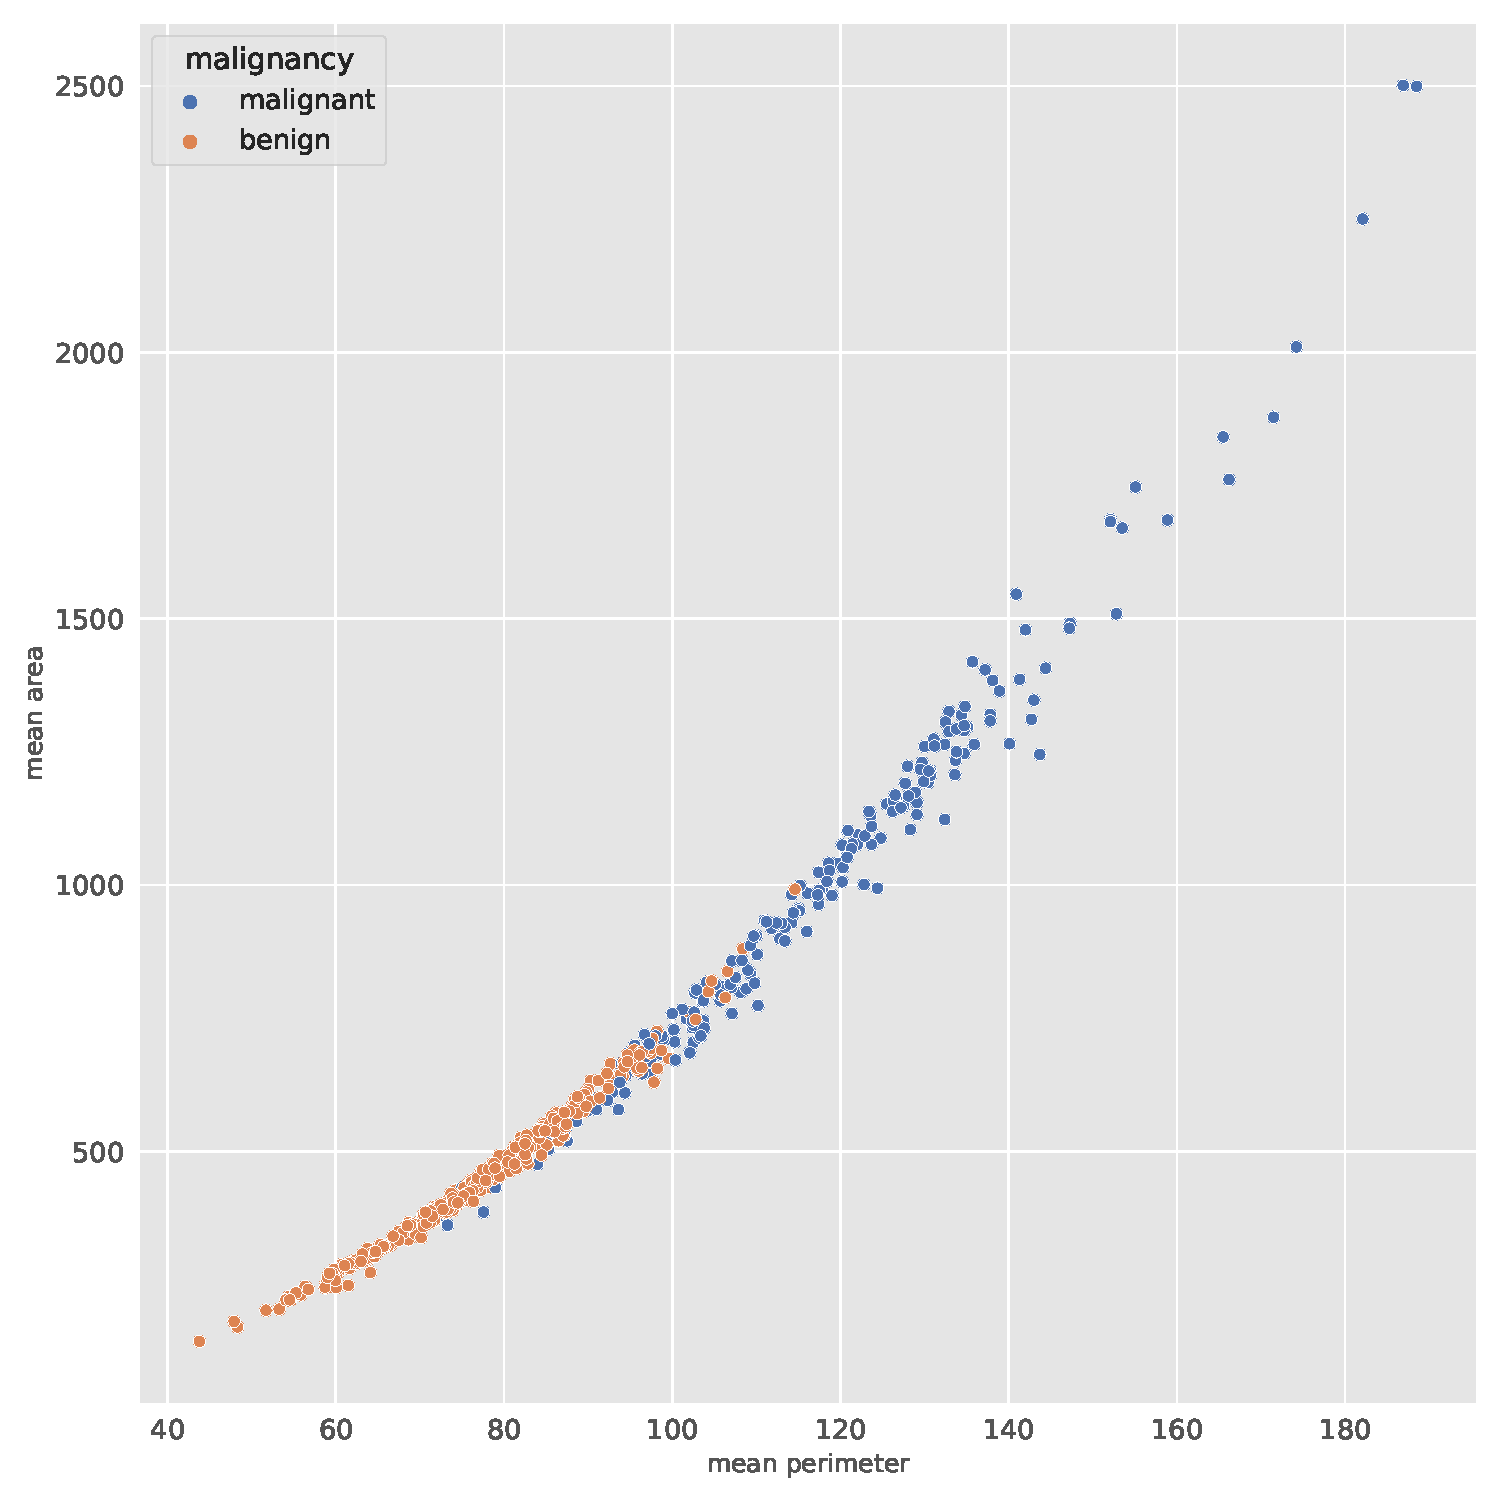
\includegraphics[scale = 0.5]{Task5/perimeterVArea.pdf}
  \caption{Perimeter Vs Area of Tumor}
  \label{fig:perimVArea}
\end{figure}

\begin{figure}[H]
  \centering
  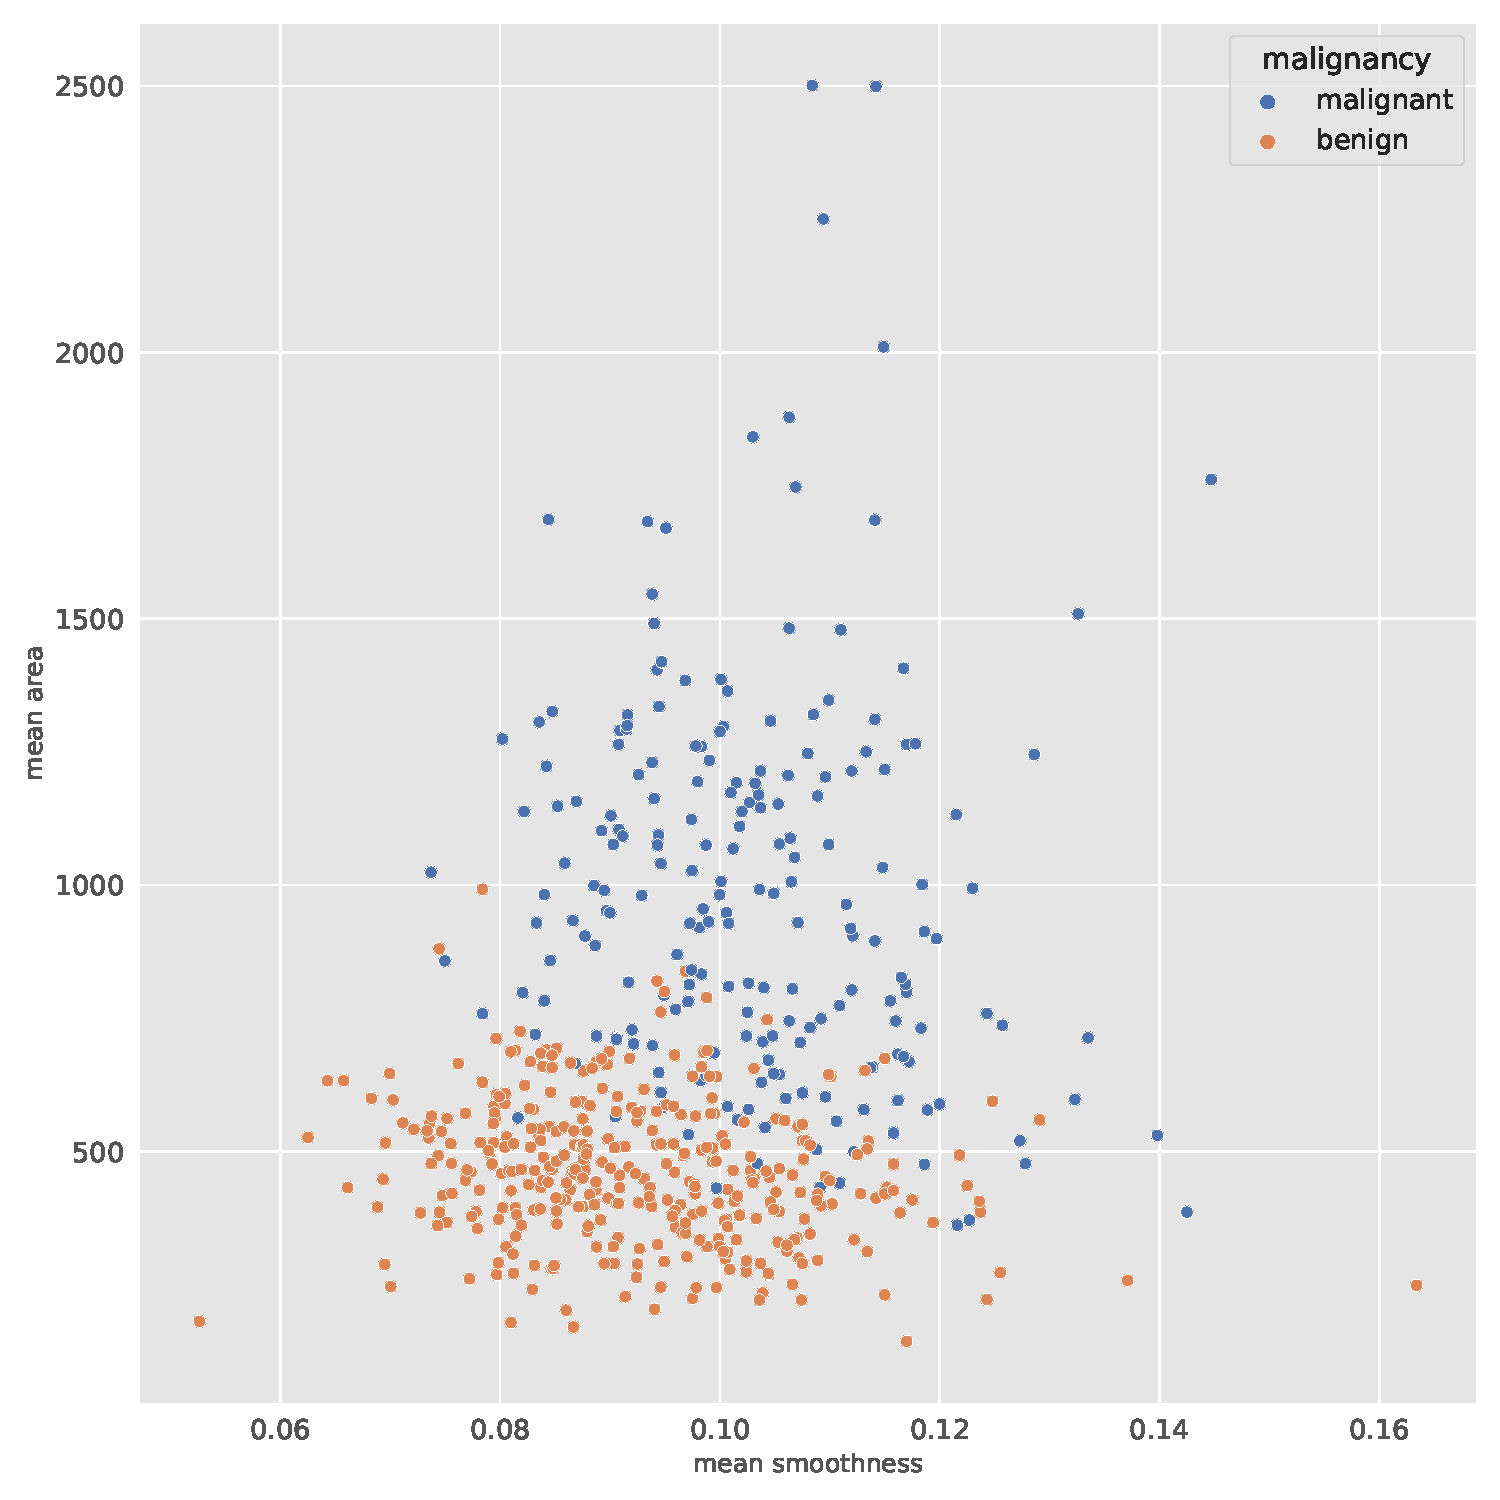
\includegraphics[scale = 0.5]{Task5/smoothVArea.pdf}
  \caption{Smoothness Vs Area of Tumor}
  \label{fig:smoothnessVArea}
\end{figure}
\begin{figure}[H]
  \centering
  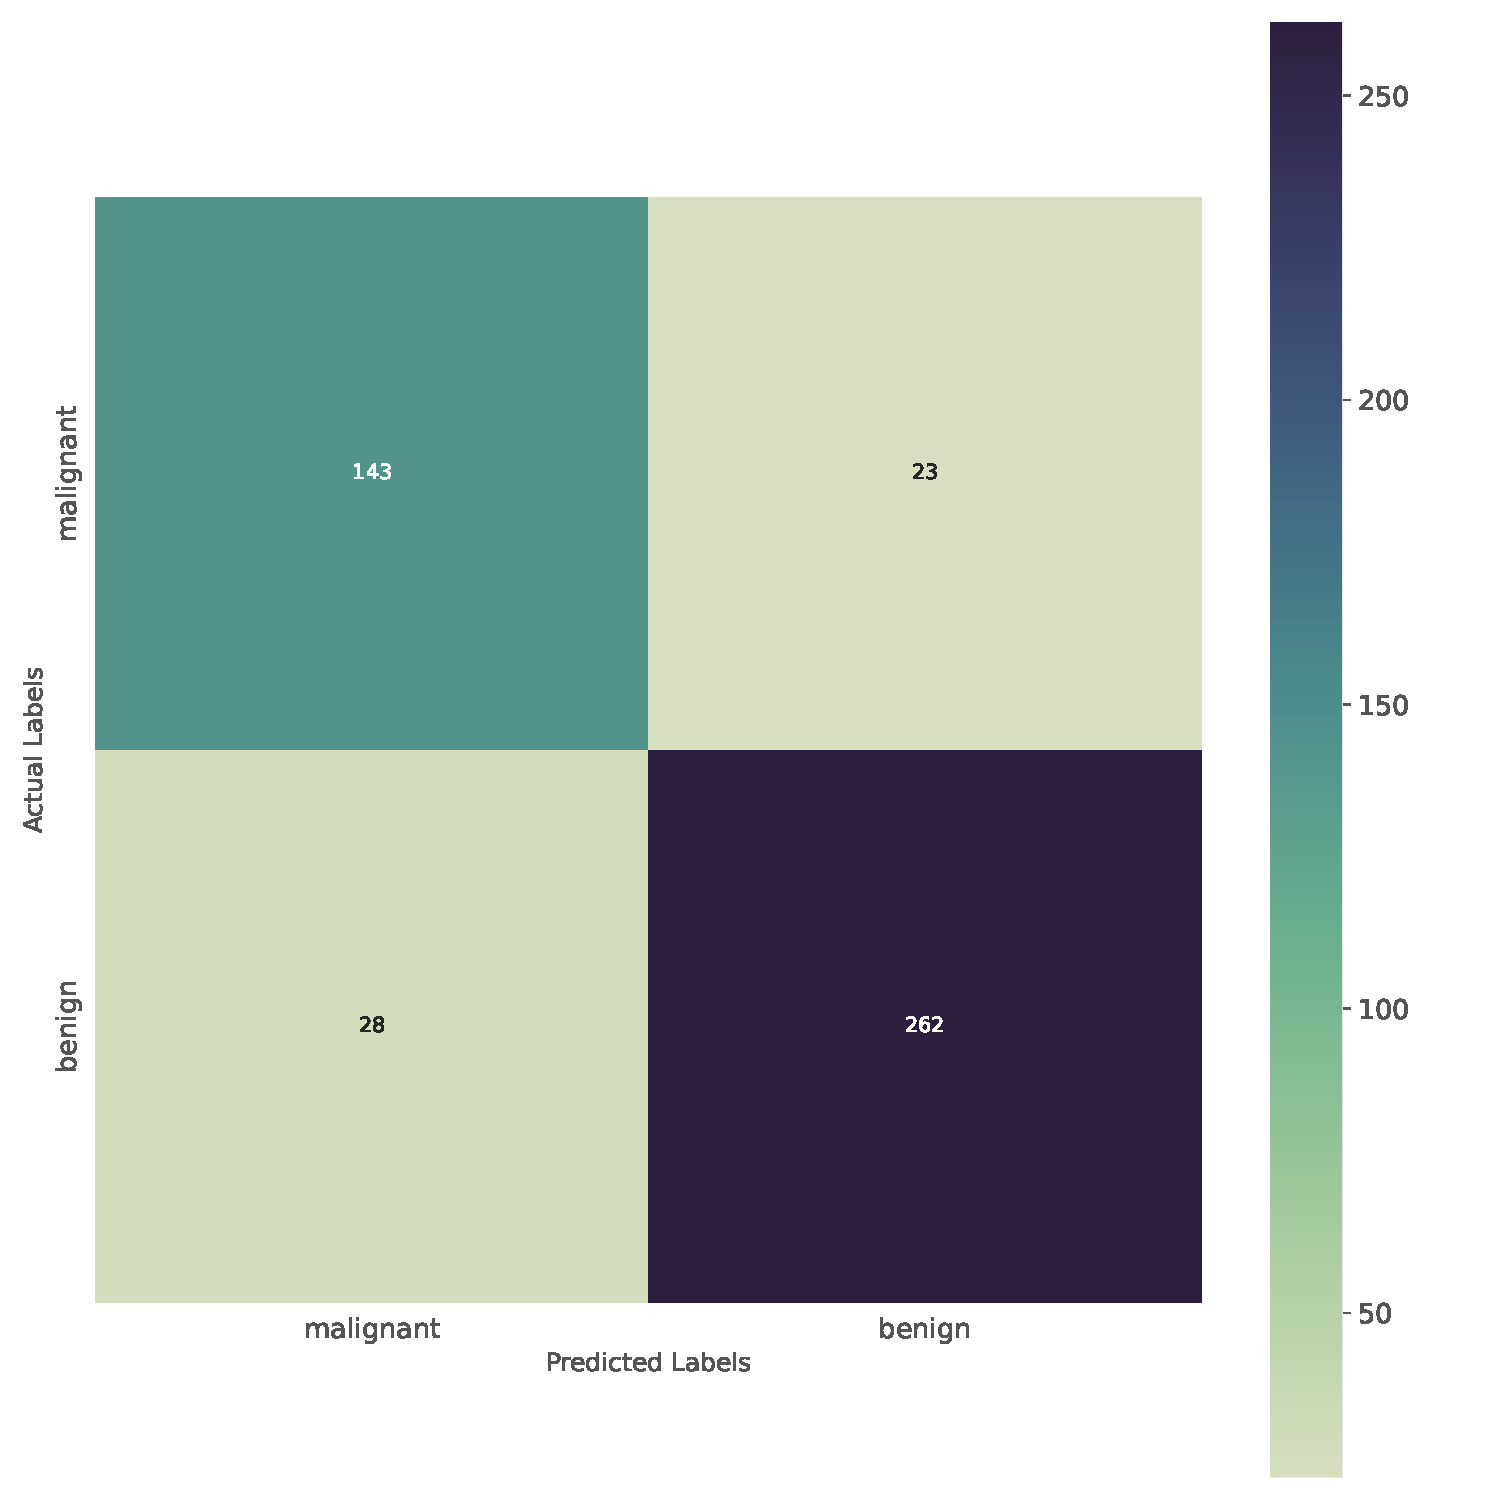
\includegraphics[scale = 0.5]{Task5/confM.pdf}
  \caption{Confusion Matrix for the Breast Cancer classifier}
  \label{fig:confM}
\end{figure}
\end{document}
